\begin{block}{Example}
\centering
    Consider an exponential decay problem with uncertain initial condition:
    \begin{equation*}
        \partial_t u = - u, \; u(t_0) = \lambda^\dagger = 0.5
    \end{equation*}

    \begin{figure}
        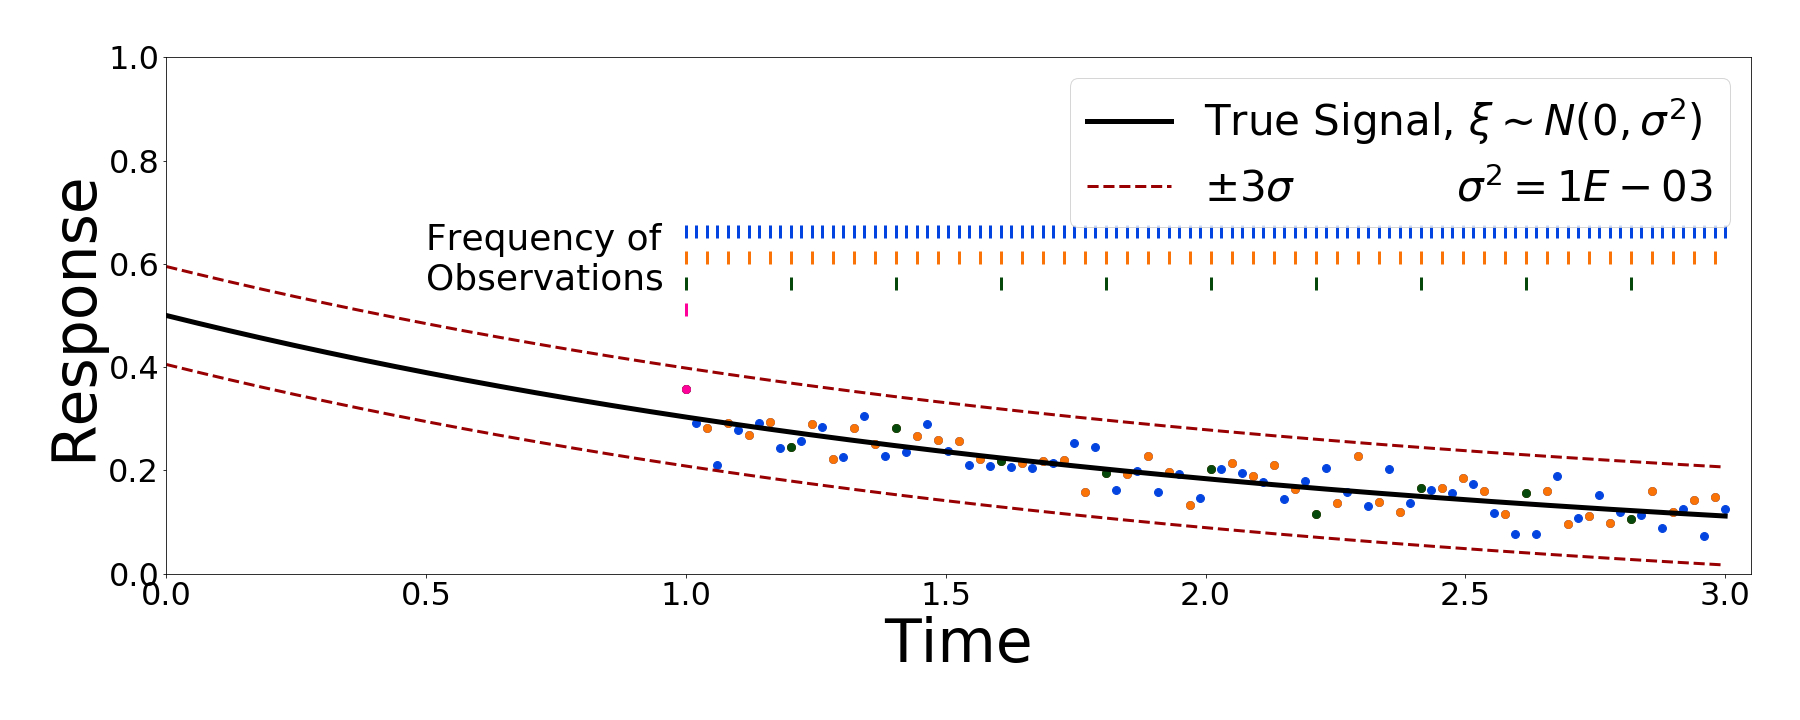
\includegraphics[height=10cm]{exponential_decay_response_sigma-10E-4}
    \end{figure}

%\end{block}

\vspace{1cm}

%\begin{block}{Convergence}
\centering
\heading{\LARGE Convergence}
\vspace{-1cm}
    \begin{figure}
        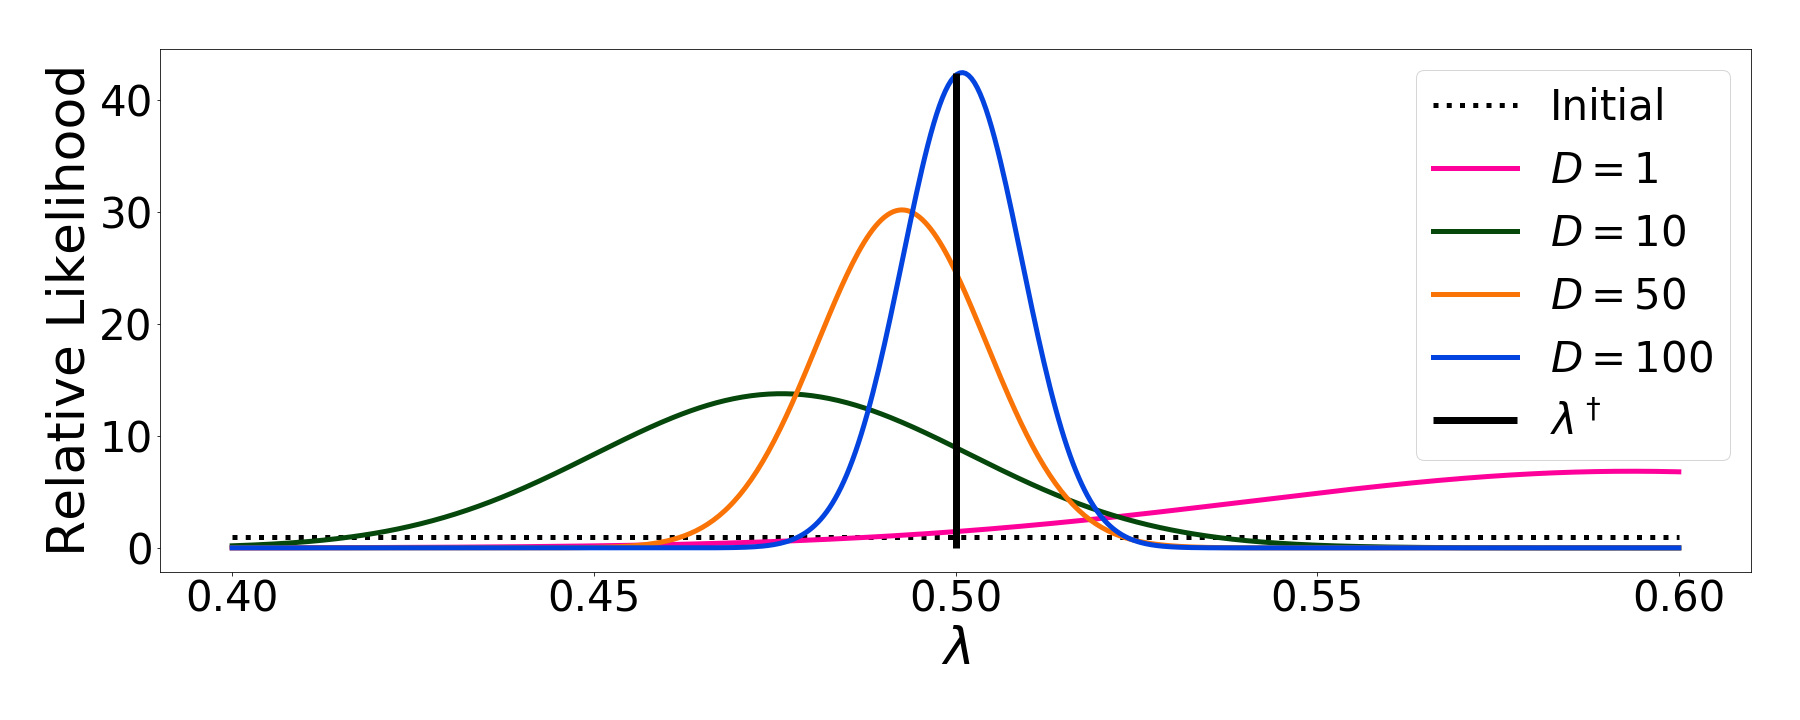
\includegraphics[height=10cm]{updated_convergence_sigma-10E-4}
        \caption*{$\param^\dagger$ and $\predicted$ for $D=1, 10, 50, 100$ for $N=1000$}
    \end{figure}

%\end{block}

\vspace{1cm}

%\begin{block}{Stability}
\heading{\LARGE Stability}
\vspace{-1cm}
    \begin{figure}
        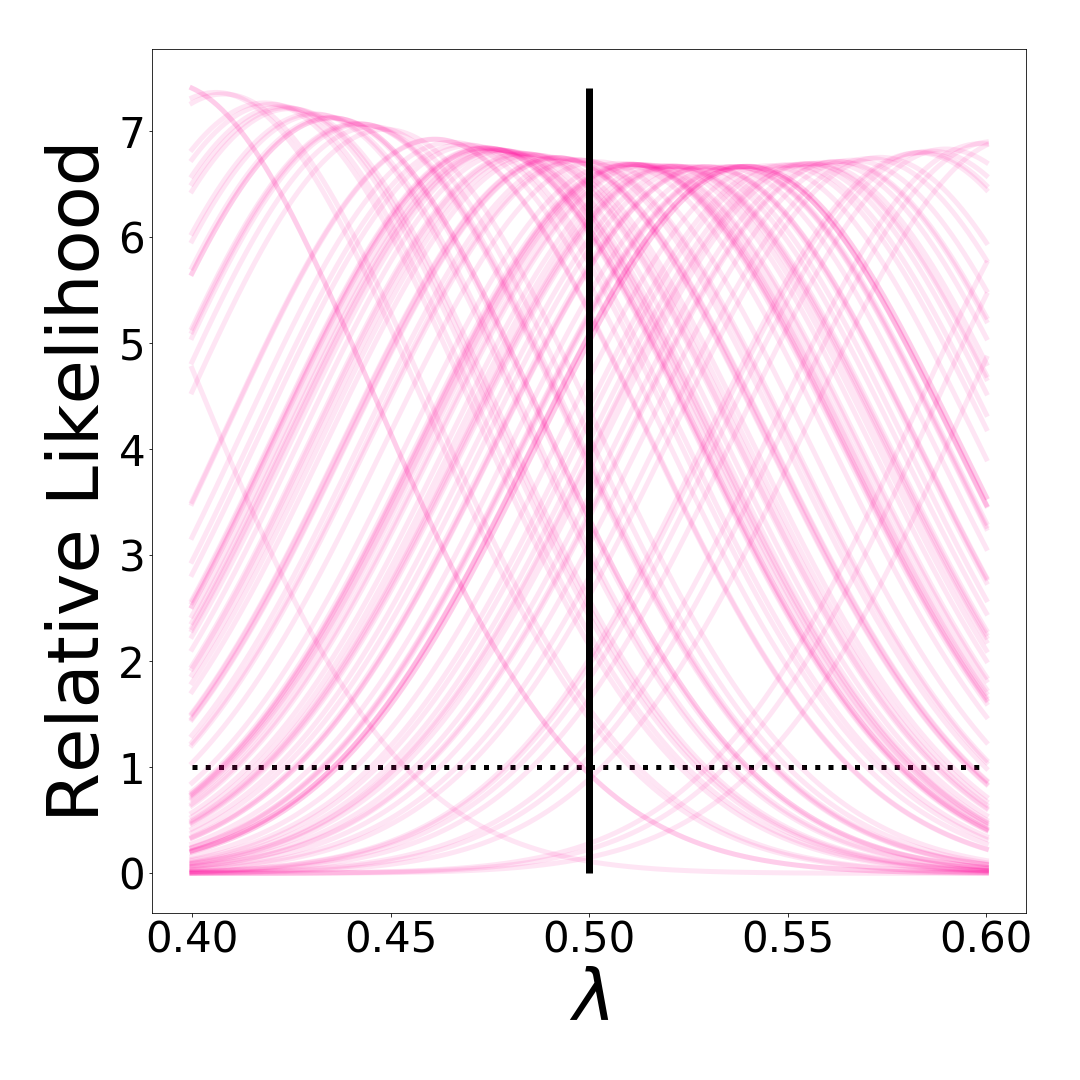
\includegraphics[width=12cm]{updated_stability_D1_sigma-10E-4}
        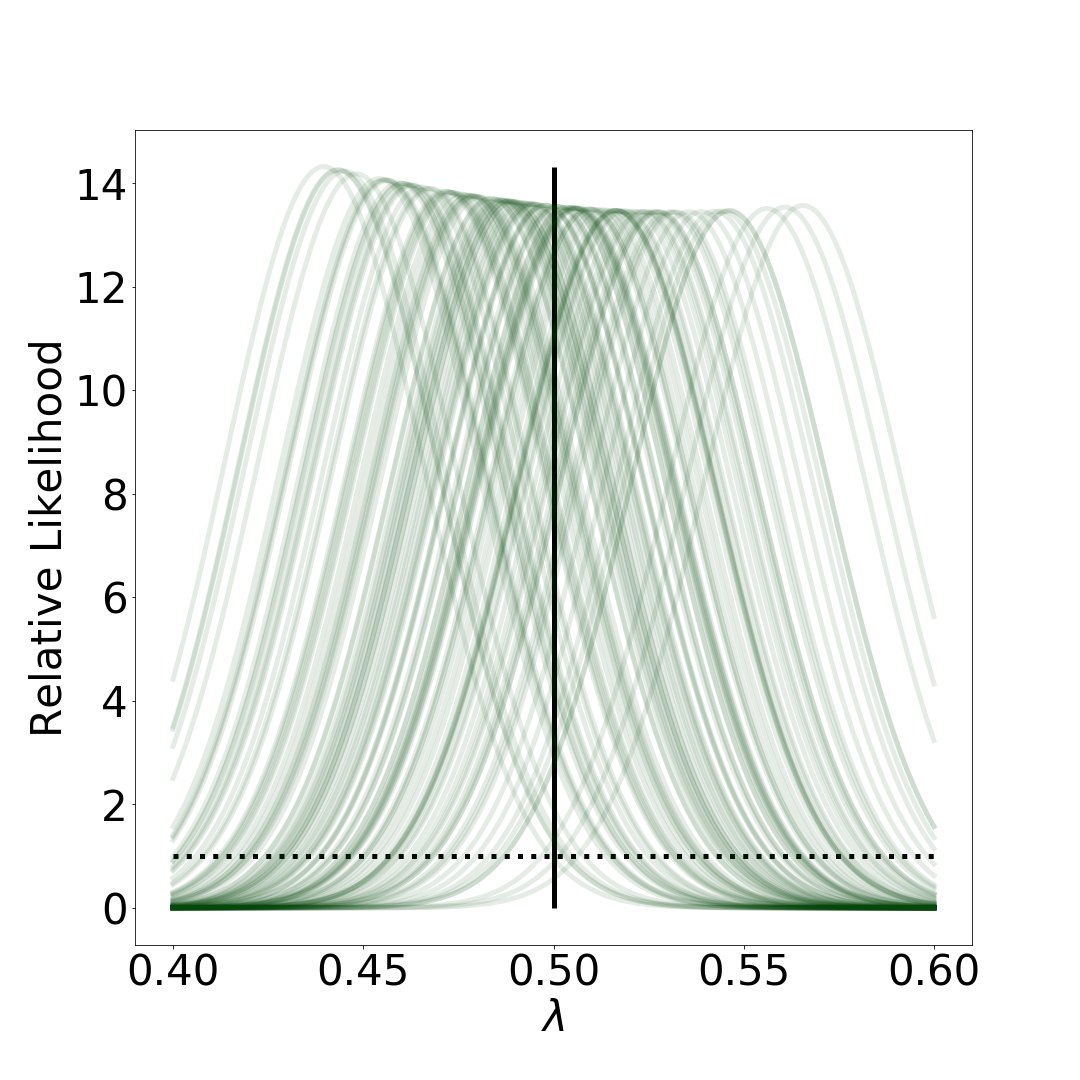
\includegraphics[width=12cm]{updated_stability_D10_sigma-10E-4}
        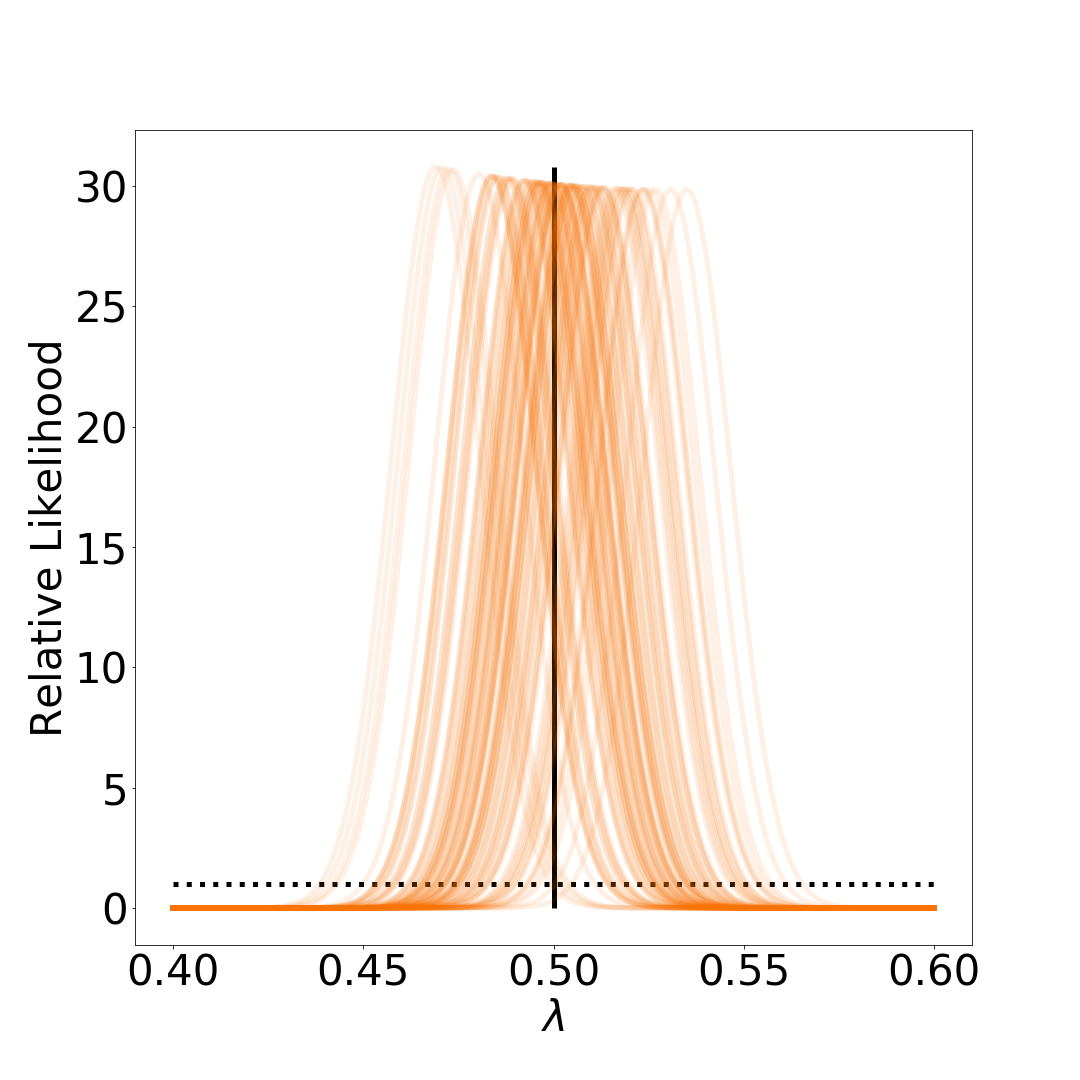
\includegraphics[width=12cm]{updated_stability_D50_sigma-10E-4}
        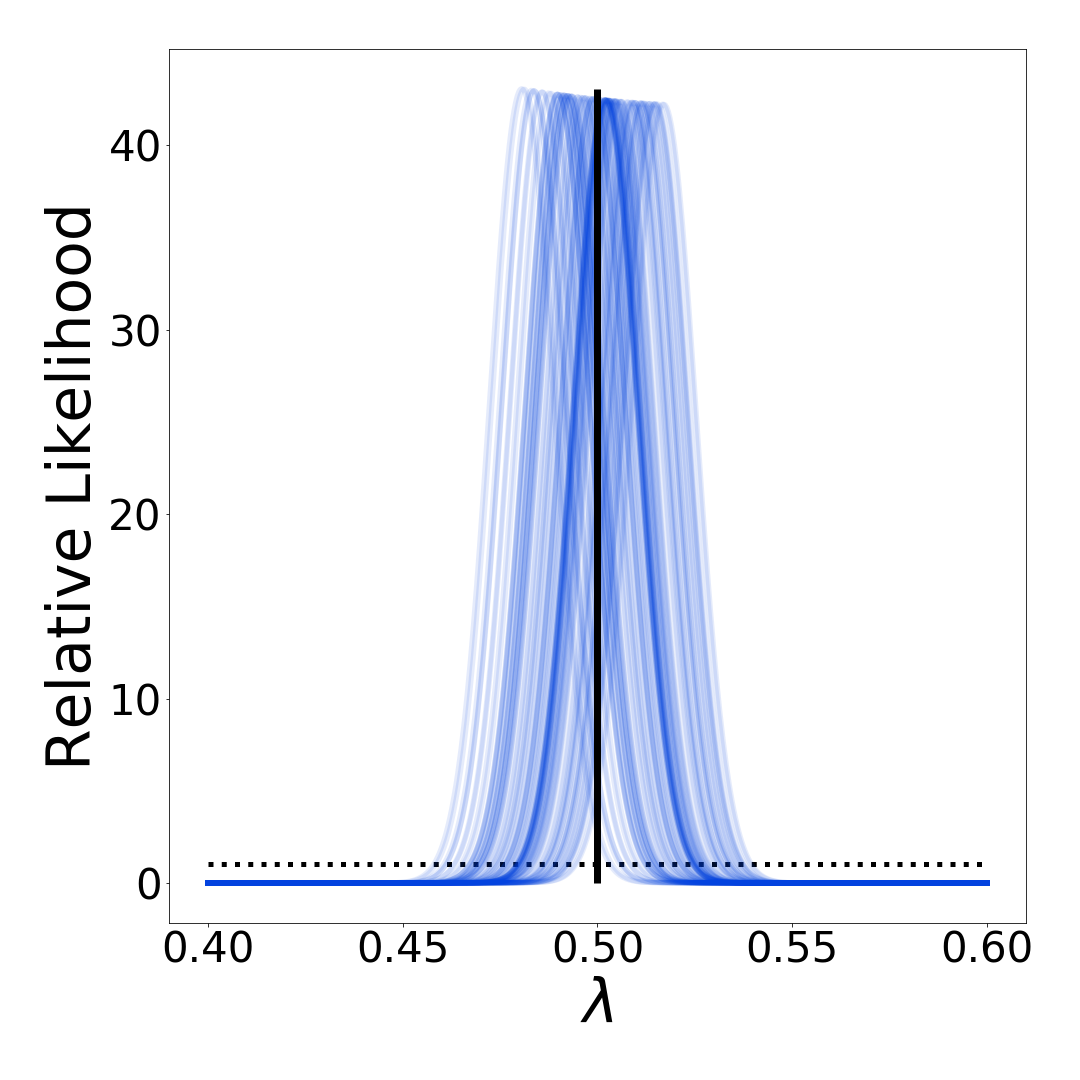
\includegraphics[width=12cm]{updated_stability_D100_sigma-10E-4}
        \caption*{$\predicted$ for one hundred realizations of $\noise^\dagger$ for $D=1, 10, 50, 100$}
    \end{figure}

\end{block}
